%==============================================================================
% Section 1 -- Introduction and State of the Art
%==============================================================================
\section{Introduction}
\label{sec:introduction}

\subsection{Novel View Synthesis}

Novel view synthesis (NVS) aims to generate photorealistic images from arbitrary
viewpoints given a set of images captured from known camera positions.
Applications include virtual reality, autonomous driving, and digital heritage
preservation. Deep learning has replaced traditional multi-view stereo methods
with learned representations, and two have emerged as state-of-the-art:
\textbf{NeRF}~\cite{mildenhall2020nerf} and \textbf{3DGS}~\cite{kerbl2023gaussian}.

%------------------------------------------------------------------------------
\subsection{Neural Radiance Fields (NeRF)}
\label{ssec:nerf}

NeRF represents a scene as a continuous volumetric function:
\begin{equation}
  F_\theta: (\mathbf{x}, \mathbf{d}) \longrightarrow (\mathbf{c}, \sigma)
\end{equation}
where $F_\theta$ is an MLP mapping position $\mathbf{x} \in \R^3$ and viewing
direction $\mathbf{d}$ to colour $\mathbf{c}$ and density $\sigma$. A pixel
colour is computed by integrating along the ray:
\begin{equation}
  \hat{C}(\mathbf{r}) = \int_{t_n}^{t_f} T(t)\,\sigma(\mathbf{r}(t))\,
    \mathbf{c}(\mathbf{r}(t),\mathbf{d})\,\mathrm{d}t, \quad
  T(t) = \exp\!\left(-\int_{t_n}^{t}\sigma(\mathbf{r}(s))\,\mathrm{d}s\right)
\end{equation}

\paragraph{Limitations.} NeRF requires 1--2 days of training and renders at
5--30 s/frame due to the cost of per-pixel MLP evaluations.

%------------------------------------------------------------------------------
\subsection{3D Gaussian Splatting (3DGS)}
\label{ssec:3dgs}

3DGS represents the scene as a set of \emph{explicit, learnable 3D Gaussian
primitives}. Each Gaussian $\Gcal_i$ stores a position $\mean_i \in \R^3$, a
covariance $\cov_i$, an opacity $o_i$, and view-dependent colour as spherical
harmonic (SH) coefficients. Rendering is performed by projecting each 3D
Gaussian onto the image plane (splatting) and compositing the resulting 2D
splats via differentiable alpha blending on the GPU, achieving $>$90 fps at
1080p. Gaussians are initialised from a SfM sparse point cloud and optimised
end-to-end with adaptive density control (Section~\ref{sec:optimization}).

%------------------------------------------------------------------------------
\subsection{Comparative Analysis: NeRF vs.\ 3DGS}
\label{ssec:comparison}

\begin{table}[H]
  \centering
  \caption{Qualitative comparison between NeRF and 3DGS.}
  \label{tab:comparison}
  \renewcommand{\arraystretch}{1.4}
  \begin{tabular}{l p{5.2cm} p{5.2cm}}
    \toprule
    \textbf{Criterion} & \textbf{NeRF} & \textbf{3D Gaussian Splatting} \\
    \midrule
    Representation     & Implicit (MLP) & Explicit (Gaussian primitives) \\
    Rendering method   & Ray casting + volume integration & GPU rasterisation (splatting) \\
    Render speed       & $<$1--30 fps & $>$90 fps (consumer GPU) \\
    Training time      & 1--2 days; 5 min (Instant-NGP) & 20--40 minutes \\
    Memory (inference) & Low (MLP weights) & High ($\sim$1 GB/scene) \\
    Editability        & Difficult & Easy (explicit geometry) \\
    \bottomrule
  \end{tabular}
\end{table}

NeRF's implicit representation handles smooth geometry naturally; 3DGS trades
spatial continuity for hardware-accelerated rendering and explicit editability.

\begin{figure}[H]
  \centering
  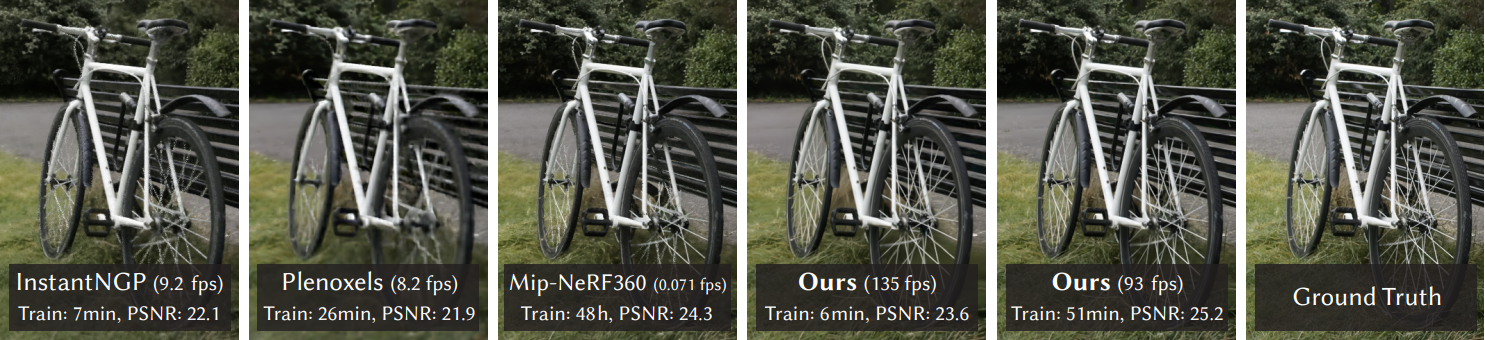
\includegraphics[width=\textwidth]{figures/3dgs_teaser.png}
  \caption{Photo-realistic novel views synthesised with 3D Gaussian Splatting at
           $>$90 fps on a consumer GPU. Each scene is reconstructed from a set of
           posed photographs; the Gaussian map supports real-time rendering from
           any viewpoint. Image from Kerbl et al.~\cite{kerbl2023gaussian}.}
  \label{fig:teaser}
\end{figure}

\medskip
The remainder of this document covers the mathematical foundations of 3DGS:
geometric representation (Sections~\ref{sec:gaussian_repr}--\ref{sec:projection}),
the rendering pipeline (Sections~\ref{sec:rasterization}--\ref{sec:alpha_blending}),
the optimisation strategy (Section~\ref{sec:optimization}), and the extension to
SLAM (Section~\ref{sec:slam}).
